\documentclass{article}

\usepackage{standalone}
\usepackage{amssymb}
\usepackage{amsbsy}
\usepackage{amsthm}
%\usepackage[dvips]{graphicx}
\usepackage{framed}
\usepackage{amsmath}

\usepackage{graphicx}

\usepackage{natbib}
\bibliographystyle{chicago}

\usepackage{subfiles}

\usepackage[final]{pdfpages}
\voffset=-1.5cm
\oddsidemargin=0.0cm
\textwidth = 470pt

\begin{document}
	\tableofcontents
\subfile{00-Intro.tex}
\subfile{00-LinearRegression.tex}
\subfile{01-Definitions.tex}
\subfile{01-Outliers.tex}
\subfile{01-outlierTest.tex}
\subfile{02-ResidualVariance.tex}
\subfile{03-residualdiagnostics.tex}
%====%
\section{Residuals and Diagnostics}

* For a given value X of the independent variable, the value predicted by regression line $\hat{y}$ is often called the \textbf{fitted
	value} of the dependent variable. 
* The difference between the observed value Y and the fitted value Y
is called the residual for that observation and is denoted by \textbf{e}:
\[e= Y-\hat{Y}\]

* (Important for later: Residuals represent unexplained (or residual) variation after fitting a regression
model. )
For the example used in this class, the residuals are very small.



\subsection{Examining the Residuals}

Recall: 

* The mean value of the residuals is zero,
* The variance of residuals are constant across the range of measurements,
* The residuals are normally distributed,
* Residuals are independent.

 
A residual plot is obtained by plotting the residuals e with respect to the independent variable X or,
alternatively with respect to the fitted regression line values $\hat{Y}$. Such a plot can be used to
investigate whether the assumptions concerning the residuals appear to be satisfied.

\subsection{Asummption of Constant Variance}

* Homoscedascity (also known as constant variance) is one of the assumptions required in a
regression analysis in order to make valid statistical inferences about population relationships.

* Homoscedasticity requires that the variance of the residuals are constant for all fitted values,
indicated by a uniform scatter or dispersion of data points about the trend line (i.e. "The Zero Line").
* From the above plot, we can conclude that the constant variance assumption is valid. We can also
see that the mean value of the residuals is close to zero. \textit{(Theoretically it is precisely zero)}.


\begin{figure}
\centering
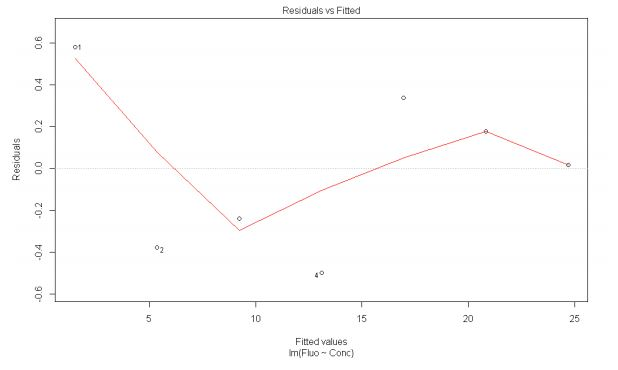
\includegraphics[width=1.1\linewidth]{ResidPlot1}
\end{figure}

\subsection{Normality of Residuals}
Additionally, the linear model approach requires this assumption that the residuals are normally
distributed. We can use a Q-Q plot to assess the normality of residuals.
\begin{figure}
\centering
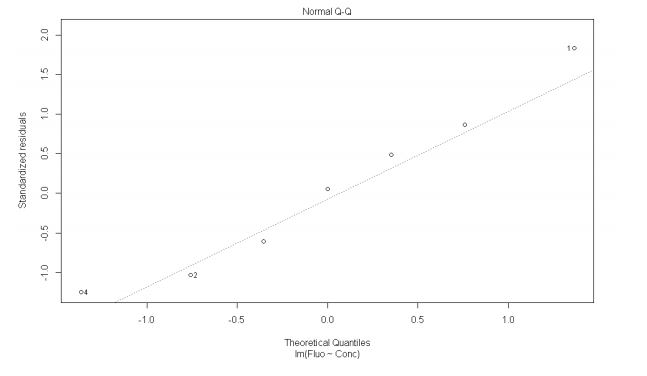
\includegraphics[width=1.1\linewidth]{ResidPlot2}
\end{figure}

<p>
\section{Regression Diagnostics}

An excellent review of regression diagnostics is provided in John Fox's aptly named \textbf{Overview of Regression Diagnostics}. Dr. Fox's car package provides advanced utilities for regression modeling.
\begin{framed}
	\begin{verbatim}
# Assume that we are fitting a multiple linear regression
# on the MTCARS data
library(car)
fit <- lm(mpg~disp+hp+wt+drat, data=mtcars)
	\end{verbatim}
\end{framed}

This example is for exposition only. We will ignore the fact that this may not be a great way of modeling the this particular set of data!

\subsection{Bivariate Outliers}

\begin{framed}
	\begin{verbatim}
	# Assessing Outliers
	outlierTest(fit) # Bonferonni p-value for most extreme obs

	\end{verbatim}
\end{framed}
\begin{framed}
	\begin{verbatim}
qqPlot(fit, main="QQ Plot") #qq plot for studentized resid 
leveragePlots(fit) # leverage plots
	\end{verbatim}
\end{framed}
leverage plot click to view

\subsection{Influential Observations}

\begin{framed}
\begin{verbatim}
# Influential Observations
# added variable plots 
av.Plots(fit)
# Cook's D plot
# identify D values > 4/(n-k-1) 
cutoff <- 4/((nrow(mtcars)-length(fit$coefficients)-2)) 
plot(fit, which=4, cook.levels=cutoff)
# Influence Plot 
influencePlot(fit,	id.method="identify", main="Influence Plot", sub="Circle size is proportial to Cook's Distance" )
\end{verbatim}
\end{framed}
av plots Cook's D plot influence plot click to view
%=== %
\subsection{Non-normality}
\begin{framed}
\begin{verbatim}
# Normality of Residuals
# qq plot for studentized resid
qqPlot(fit, main="QQ Plot")

# distribution of studentized residuals
library(MASS)
sresid <- studres(fit) 
hist(sresid, freq=FALSE, 
main="Distribution of Studentized Residuals")
xfit<-seq(min(sresid),max(sresid),length=40) 
yfit<-dnorm(xfit) 
lines(xfit, yfit)
\end{verbatim}
\end{framed}
qq plot histogram of studentized residuals click to view
%= %
\section{Non-constant Error Variance}

Evaluate homoscedasticity
\begin{framed}
\begin{verbatim}
# non-constant error variance test
ncvTest(fit)
# plot studentized residuals vs. fitted values 
spreadLevelPlot(fit)
spread vs. levels click to view
\end{verbatim}
\end{framed}
%= %
Multi-collinearity
\begin{framed}
\begin{verbatim}
# Evaluate Collinearity
vif(fit) # variance inflation factors 
sqrt(vif(fit)) > 2 # problem?
\end{verbatim}
\end{framed}
%==== %
\subsection{Nonlinearity}
\begin{framed}
	\begin{verbatim}
# Evaluate Nonlinearity
# component + residual plot 
crPlots(fit)
# Ceres plots 
ceresPlots(fit)
\end{verbatim}
\end{framed}
component plus residual plot Ceres plots click to view
%== %
\section{Non-independence of Errors}

The Durbin–Watson statistic is a test statistic used to detect the presence of autocorrelation (a relationship between values separated from each other by a given time lag) in the residuals (prediction errors) from a regression analysis. It is named after James Durbin and Geoffrey Watson.
\begin{framed}
	\begin{verbatim}
# Test for Autocorrelated Errors
durbinWatsonTest(fit)
\end{verbatim}
\end{framed}
\end{document}

# Assessing Outliers
outlierTest(FitAll) # Bonferonni p-value for most extreme obs
qqPlot(FitAll, main="QQ Plot") #qq plot for studentized resid 
leveragePlots(FitAll) # leverage plots
leverage plot click to view
Influential Observations
# Influential Observations
# added variable plots 
av.Plots(FitAll)
# Cook's D plot
# identify D values > 4/(n-k-1) 
cutoff <- 4/((nrow(mtcars)-length(FitAll$coefficients)-2)) 
plot(FitAll, which=4, cook.levels=cutoff)
# Influence Plot 
influencePlot(FitAll,	id.method="identify", main="Influence Plot", sub="Circle size is proportial to Cook's Distance" )
av plots Cook's D plot influence plot click to view
Non-normality
# Normality of Residuals
# qq plot for studentized resid
qqPlot(FitAll, main="QQ Plot")
# distribution of studentized residuals
library(MASS)
sresid <- studres(FitAll) 
hist(sresid, freq=FALSE, 
main="Distribution of Studentized Residuals")
xFitAll<-seq(min(sresid),max(sresid),length=40) 
yFitAll<-dnorm(xFitAll) 
lines(xFitAll, yFitAll)
qq plot histogram of studentized residuals click to view
Non-constant Error Variance
# Evaluate homoscedasticity
# non-constant error variance test
ncvTest(FitAll)
# plot studentized residuals vs. FitAllted values 
spreadLevelPlot(FitAll)
spread vs. levels click to view
Multi-collinearity
# Evaluate Collinearity
vif(FitAll) # variance inflation factors 
sqrt(vif(FitAll)) > 2 # problem?
Nonlinearity
# Evaluate Nonlinearity
# component + residual plot 
crPlots(FitAll)
# Ceres plots 
ceresPlots(FitAll)
component plus residual plot Ceres plots click to view
Non-independence of Errors
# Test for Autocorrelated Errors
durbinWatsonTest(FitAll)
